\documentclass[a4paper,10pt]{article}
\usepackage[utf8]{inputenc}
\usepackage[UKenglish]{babel}
\usepackage{fancyhdr}
\usepackage{anysize}
\usepackage{amsmath, amsthm, amssymb}
\usepackage{lastpage}
\usepackage[all]{xy}  % drawings
%\usepackage{listings} % code highlighting
\usepackage[usenames,dvipsnames]{color}
\usepackage{graphicx}
\usepackage{caption}
\usepackage{subfigure}

\pagestyle{fancy}
\fancyfoot[R]{\em \thepage / \pageref{LastPage}}
\fancyfoot[C]{}
\fancyfoot[L]{\em Master VIBOT}
\fancyhead[R]{\em Lab2 - Line features with Split \& Merge}
\fancyhead[C]{}
\fancyhead[L]{\em Probabilistic Robotics}
\renewcommand{\headrulewidth}{0.4pt}
\renewcommand{\footrulewidth}{0.4pt}

%\,	 a small space
%\:	 a medium space
%\;	 a large space
%\quad	 a really large space
%\qquad	 a huge space
%\!	 a negative space (moves things back to the left)
        
\begin{document}

\marginsize{2cm}{2cm}{2cm}{2cm}

% Title
%\hspace{1mm}
\begin{center}
\Large \textbf{Lab2 - Line features with Split \& Merge}
\end{center}
%\hspace{1mm}

\section{Introduction}

This lab is designed to learn how to extract line features from point data. The data is extracted from the \texttt{sensor\_msgs/LaserScan} messages saved in a bagfile dataset and are converted to $(x,y)$ points in a 2D plane. Your goal is to create an algorithm that creates lines from the given points. The Split \& Merge algorithm explained in the attached scientific paper will be the base of its implementation.

The resulting algorithm will be used on the following labs as a base for feature extraction in Particle Filter, Extended Kalman Filter and Simultaneous Localization and Mapping. 

\section{Pre-lab}

Read and understand the Split \& Merge algorithm explained in the attached paper. Instead of fitting a line to all points, we are going to implement the \emph{Iterative-End-Point-Fit} for its simplicity.

Lines will be represented in the form \eqref{line} because simplifies operations.

\begin{equation}
    a x + b y + c = 0 \label{line}
\end{equation}

\noindent
The questions for the prelab (answer in UdG moodle) are:

\begin{itemize}
    \item Given two points $(x_1, y_1)$ and $(x_2, y_2)$, compute the line parameters $(a,b,c)$.
    \item Given a line $(a,b,c)$ and a point $(x,y)$ compute the distance from the point to the line.
\end{itemize}

\noindent
Answer with a single formula containing only the given data.

\section{Lab work}

The ROS package \texttt{lab2\_splitandmerge} (from the metapackage \texttt{probabilistic\_labs} that you cloned during the lab0) contains all necessary code for running this lab (it is recommendable to pull the last version from the repository before starting the lab). Test the code using the following command:

\begin{verbatim}
    roslaunch lab2_splitandmerge lab2_splitandmerge.launch
\end{verbatim}

This will playback the data recorded into the bagfile \texttt{probabilistic\_basics/bags/dataset3.bag} and two nodes. One will handle the odometry of the robot (\texttt{lab2\_splitandmerge/src/odometrynode.py}) and the other one handling the laser scan data (\texttt{lab2\_splitandmerge/src/splitandmergenode.py}).

As you can see the dummy Split \& Merge algorithm implemented, only provides lines from the first to the last point of each scan without any other computation. Also you can observe how
the odometry is not perfect and the accumulation of the scans does not represent properly the map (Fig.~\ref{map}).

\begin{center}
	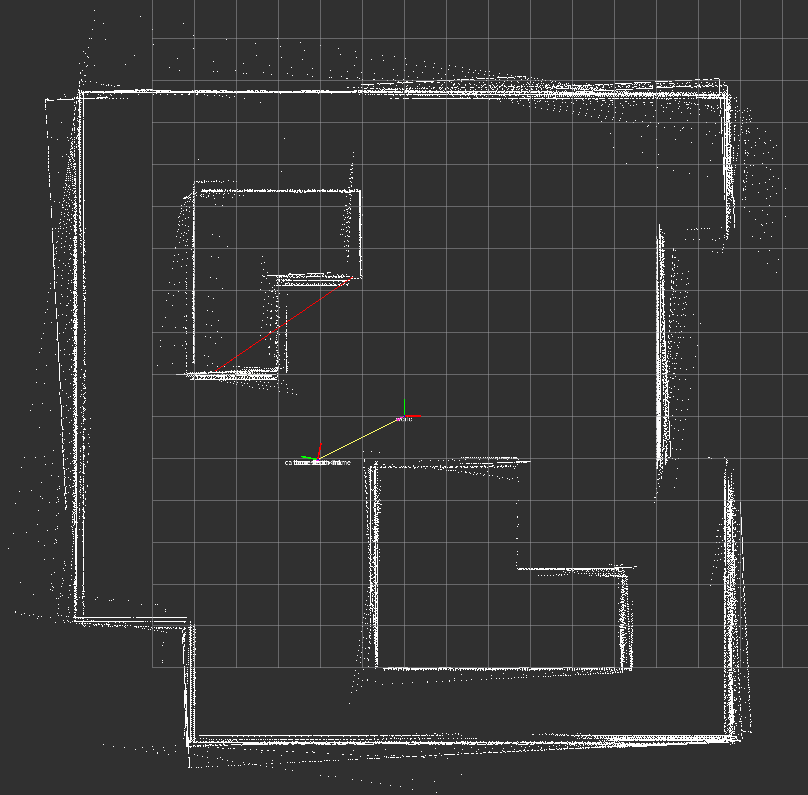
\includegraphics[width=0.5\textwidth]{scans_dataset3}
	\captionof{figure}{All points plotted with respect to odometry (white) and the line from the Split \& Merge.}
	\label{map}
\end{center}

For completing the lab you have to modify the file \texttt{lab2\_splitandmerge/src/splitandmerge.py}. The functions that have to be modified are highlighted. You can tune the parameters of the Split \& Merge algorithm by changing the values assigned by default when the \texttt{splitandmerge} function is called.

For viewing properly each scan in Rviz, decrease the \texttt{LaserScan} decay time to 0, so it will only show the last published scan. Also change the fixed frame to \texttt{camera\_depth\_frame} to see the position of the robot fixed.

\section{Optional}
\begin{itemize}
    \item Test the algorithm with both datasets \texttt{probabilistic\_basics/bags/dataset3.bag} (the one by default) and \texttt{probabilistic\_basics/bags/dataset2.bag}.
    
    (You will need to modify the file:    \texttt{launch/lab2\_splitandmerge.launch}).
    \item Represent all the lines that have been obtained by the Split \& Merge algorithm in a single image, showing the discrepancies caused by the odometry.
\end{itemize}

\section{Lab report}

Write a brief report (to be submitted in a pdf of maximum 3 pages) explaining your solution and problems faced. Include only the final \texttt{splitandmerge.py} file for us to test. If you have tested it with both datasets and different parameters are needed leave the \texttt{splitandmerge.py} with the parameters for \texttt{dataset3.bag} and report the ones used for \texttt{dataset2.bag} in the submitted pdf. The deadline for the submission of this lab is March 14th at 23:55.

\end{document}
